\documentclass[11pt]{article}

\usepackage{fullpage} 
\usepackage{hyperref}
\usepackage{amsmath}
\usepackage{amssymb}
\usepackage{amsthm}
\usepackage{graphicx}
\usepackage{pgf}
\usepackage{tikz}
\usetikzlibrary{arrows,automata}


\newcommand{\question}[2] {\vspace{0.3in}\noindent{\subsection*{Question #1. #2} \vspace{0.15in}}}

\renewcommand{\part}[1] {{\vspace{0.15in}\noindent\textbf (#1)} \vspace{0.10in}}



%  ----------------------------------------------------------------
%                         Start here
% ----------------------------------------------------------------
 
\begin{document}

\title{Assignment \#1} %Replace X with the appropriate number
\author{\Large Gustavo Estrela de Matos\\ %Replace with your name
CSCE 433: Formal Languages and Automata} %If necessary, replace with your course number and title
\date{\today}
\maketitle


\question{1}{Prove by induction that for $n \ge 1$, $\sum_{i = 1}^{n}\frac{1}{2 ^ i} = 1 - \frac{1}{2^n}$}
\begin{itemize}
\item{Base case:} For the base case we know that $n = 1$, then: \\
    $\sum_{i = 1}^{1}{\frac{1}{2^i}} = {\frac{1}{2}}$; and also $1 - {\frac{1}{2}} = {\frac{1}{2}}$.\\
    Therefore the equation holds for the base case.
\item{Inductive hypothesis:} Assume that the equation holds for $2 \leq n \leq k$ for some integer $k$
\item{Inductive step:} For the case where $n = k + 1$, we have that: 
\begin{equation*}
\begin{aligned}
    \sum_{i = 1}^{k + 1}{\frac{1}{2^i}} & = \sum_{i = 1}^{k}{\frac{1}{2^i}} + {\frac{1}{2^{k + 1}}} \\
                                        & = 1 - \frac{1}{2^k} + \frac{1}{2^{k + 1}} \textup{ (by inductive hypothesis)} \\
                                        & = 1 - (\frac{1}{2^k})(1 - \frac{1}{2}) \\
                                        & = 1 - \frac{1}{2^{k + 1}} \\
\end{aligned}
\end{equation*}
    Then, if the equations holds for $k$ it also holds for $k + 1$. Now by induction, using the base case, inductive hypothesis and inductive step, we have that for all $n \geq 1$ the equation holds, as we wanted to proof.

\end{itemize}


\question{2}{Show that any integer postage greater than 7 cents can be formed by using only 3-cent and 5-cent stamps}
Basically, what we want to demonstrate is that, for any $n > 7$, $n$ can be written as 
\begin{align}
    n = 3a + 5b \label{eq2}
\end{align}
where $a$ and $b$ non negative numbers. Let $k$ be an integer such that $k > 7$ and take $k \mod 3$:
\begin{itemize}
\item{if $k \equiv 0 \mod 3$:} \\
    Then, for some integer $q \geq 0$, $k = 3q$, so equation \ref{eq2} holds.

\item{if $k \equiv 1 \mod 3$:} \\
    We have that
\begin{equation*}
\begin{aligned}
    k - 10 &\equiv 1 - 10 \mod 3\\
    k - 10 &\equiv 0 \mod 3 
\end{aligned}
\end{equation*}
    and, since $k > 7$ and $k \equiv 1 \mod 3$ we have that $k \geq 10$, hence $k - 10 \geq 0$ and there is $q \geq$ integer such that
\begin{equation*}
\begin{aligned}
    k - 10 &= 3q \\
    k      &= 3(q) + 5(2) \\
\end{aligned}
\end{equation*}
    Therefore, equation \ref{eq2} also holds for this case.

\item{if $k \equiv 2 \mod 3$:} \\
    We have that
\begin{equation*}
\begin{aligned}
    k - 5 &\equiv 2 - 5 \mod 3\\
    k - 5 &\equiv 0 \mod 3 
\end{aligned}
\end{equation*}
    and, since $k > 7$, there is $q \geq 0$ integer such that
\begin{equation*}
\begin{aligned}
    k - 5 &= 3q \\
    k &= 3(q) + 5(1) 
\end{aligned}
\end{equation*}
    Therefore, equation \ref{eq2} holds again.
\end{itemize}
Since the equation \ref{eq2} holds for all cases it holds for any case.

\question{3}{Give a DFA for each of the following languages}

\textbf{\part{a} Binary strings that contais at least five 1s.}

\begin{itemize}
	\item $Q = \{q_0, q_1, q_2, q_3, q_4, q_5\}$,	
	\item $\Sigma = \{0,1\}$,
	\item $q = q_0$,
	\item $F = \{q_5\}$, and
        \item $\delta$ is defined as follows

\begin{tabular}{|c||c|c|}  \hline
      & 0 & 1 \\ \hline 
      $q_0$ & $q_0$ & $q_1$ \\ \hline 
      $q_1$ & $q_1$ & $q_2$ \\ \hline
      $q_2$ & $q_2$ & $q_3$ \\ \hline
      $q_3$ & $q_3$ & $q_4$ \\ \hline 
      $q_4$ & $q_4$ & $q_5$ \\ \hline 
      $q_5$ & $q_5$ & $q_5$ \\ \hline 
\end{tabular}

\end{itemize}
\begin{figure}[h]
\centering
\fbox{
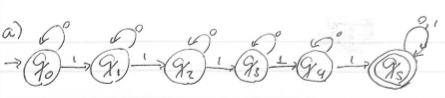
\includegraphics{dfa-a.png}
}
\end{figure}
In this machine, the state $q_i$, $ 0 \leq i \leq 4$ , represents that the string read has $i$ 1s. The state $q_5$ represents that the string has $5$ or more 1s.
\newline
\newline\textbf{\part{b} Binary strings that beggins with 010 or ends with 101}

\begin{itemize}
	\item $Q = \{q_0, q_1, q_2, q_4, q_5, q_6, q_7, q_8\}$,	
	\item $\Sigma = \{0,1\}$,
	\item $q = q_0$,
	\item $F = \{q_4, q_8\}$, and
        \item $\delta$ is defined as follows.

\begin{tabular}{|c||c|c|}  \hline
      & 0 & 1 \\ \hline 
      $q_0$ & $q_1$ & $q_5$ \\ \hline 
      $q_1$ & $q_7$ & $q_2$ \\ \hline
      $q_2$ & $q_4$ & $q_5$ \\ \hline
      $q_4$ & $q_4$ & $q_4$ \\ \hline 
      $q_5$ & $q_6$ & $q_5$ \\ \hline 
      $q_6$ & $q_7$ & $q_8$ \\ \hline 
      $q_7$ & $q_7$ & $q_5$ \\ \hline 
      $q_8$ & $q_6$ & $q_5$ \\ \hline 
\end{tabular}
\end{itemize}

\begin{figure}[h]
\centering
\fbox{
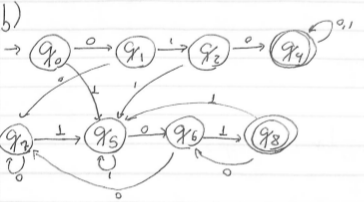
\includegraphics{dfa-b.png}
}
\end{figure}
The states $q_i$, $0 \leq i \leq 4$ are states that verify if the string starts with 010. If this fails, the machine goes to the states bellow which are responsible for verifying if the string ends with 101.

\textbf{\part{c} Binary strings having the substring 010 but not having the substring 101}
\begin{itemize}
	\item $Q = \{q_0, q_1, q_2, q_3, q_4, q_5, q_6, q_7\}$,	
	\item $\Sigma = \{0,1\}$,
	\item $q = q_0$,
	\item $F = \{q_4, q_5, q_8, q_9\}$, and
        \item $\delta$ is defined as follows.

\begin{tabular}{|c||c|c|}  \hline
      & 0 & 1 \\ \hline 
      $q_0$ & $q_1$ & $q_2$ \\ \hline 
      $q_1$ & $q_1$ & $q_3$ \\ \hline
      $q_2$ & $q_6$ & $q_2$ \\ \hline
      $q_3$ & $q_4$ & $q_2$ \\ \hline 
      $q_4$ & $q_5$ & $q_7$ \\ \hline 
      $q_5$ & $q_5$ & $q_8$ \\ \hline 
      $q_6$ & $q_1$ & $q_7$ \\ \hline 
      $q_7$ & $q_7$ & $q_7$ \\ \hline 
      $q_8$ & $q_9$ & $q_8$ \\ \hline 
      $q_9$ & $q_5$ & $q_7$ \\ \hline 
\end{tabular}
\end{itemize}
The states $q_1$ and $q_3$ are responsible for verifying if the string has substring 010, and once this is checked the machine stays in the states $q_4, q_5, q_8 and q_9$ as long as the string 101 is not read. If the substring 101 appears before 010 the machine goes to state $q_7$ through the states $q_2$ and $q_6$.
\begin{figure}[h]
\centering
\fbox{
    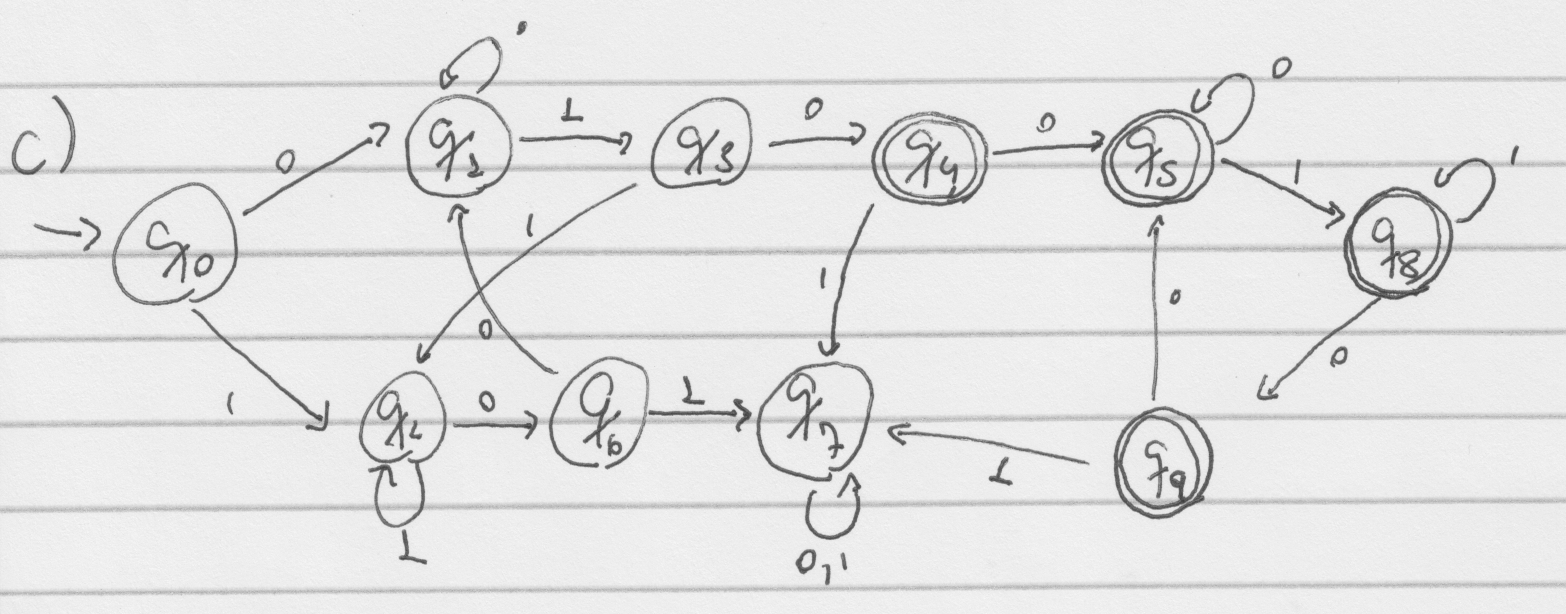
\includegraphics[scale=0.2]{dfa-c.png}
}
\end{figure}
\end{document}

